% Created 2018-10-27 Sat 19:34
% Intended LaTeX compiler: pdflatex
\documentclass[11pt]{article}
\usepackage[utf8]{inputenc}
\usepackage[T1]{fontenc}
\usepackage{graphicx}
\usepackage{grffile}
\usepackage{longtable}
\usepackage{wrapfig}
\usepackage{rotating}
\usepackage[normalem]{ulem}
\usepackage{amsmath}
\usepackage{textcomp}
\usepackage{amssymb}
\usepackage{capt-of}
\usepackage{hyperref}
\usepackage{color}
\usepackage{minted}
\usepackage{color}
\usepackage{minted}
\usepackage{parskip}
\usepackage{geometry}
\geometry{left=2.5cm,right=2.5cm,top=2.5cm,bottom=2.5cm}
\author{Daniel Moreno Manzano}
\date{\today}
\title{Quantum Volume}
\hypersetup{
 pdfauthor={Daniel Moreno Manzano},
 pdftitle={Quantum Volume},
 pdfkeywords={},
 pdfsubject={},
 pdfcreator={Emacs 25.1.1 (Org mode 9.1.14)}, 
 pdflang={English}}
\begin{document}

\maketitle

\section{Introduction}
\label{sec:orgeee1eb6}

Given the different hardware implementations and technologies in Quantum Computation (superconducting, ion-trap, spin qubits, \ldots{}), it is often difficult to benchmark the usefulness or power of quantum systems. 
A \textbf{hardware-independent measure} is required to depict whether a device is able to run a quantum circuit or not.
Here is where the Quantum Volume metric appears on the scene.

The aim of Quantum Volume is to quantify the computational power of quantum devices. 
Consequently we will use it as a metric to measure the runnability of the quantum algorithms and the quantum devices -- \emph{\textbf{"can this algorithm be run in a given device?"}}.
While the device is the basis of the Quantum Volume metric, we fix our attention on the circuit.
Our purpose is to assert how the mapping procedure affects the runnability of a given circuit and to study how the Quantum Volume is related to the probability of success.

\section{Quantum Volume definition}
\label{sec:orgf71e85a}

In this section, we define the Quantum Volume metric as well as the insights and ideas motivated by its capabilities

\subsection{Literature review}
\label{sec:orgf684356}

Few studies have been published on the Quantum Volume topic \cite{Bishop_2017,Moll_2018}.
In this section, a brief introduction to the metric is offered, reviewing the important concepts and basis.

\subsubsection{Hardware parameters}
\label{sec:orgf97d927}

The Quantum Volume metric considers that a quantum computer's performance mainly depends on the next hardware specifications:

\begin{itemize}
\item \(N\). The number of physical qubits
\item Quantum chip topology. The connectivity between qubits
\item Maximum number of sequential gates with correctable errors. The number of gates that can be applied before errors or decoherence mask the result
\item Gate set. Available hardware gate set
\item Maximum number of parallel operations. Number of operations that can be run in parallel
\end{itemize}

\subsubsection{Definitions and metrics}
\label{sec:orgdd47925}

In order to understand the metric of Quantum Volume, some concepts need to be defined first. 
In this section we offer the inferred definitions from \cite{Bishop_2017,Moll_2018} that are part of the rationale of Quantum Volume.


\begin{description}
\item[{Model algorithm.}] In the literature, Bishop et al. use the term \emph{model algorithm} in \cite{Bishop_2017} to refer to a depth-one circuit, "constructed by random 2-qubit unitary matrix chosen uniformly over \(SU (4)\) on a random pairing of the qubits". Or, what is the same, the \emph{model algorithm} is a \emph{circuit unit} defined by a combination of any single- or two-qubit gates. The mapping requirements of the device and the mapping quality is included as well. In the case that a two-qubit gate force any qubit to be routed, the gate additions will be included in the \emph{model algorithm}. Therefore, we can say that the it is a device specific metric, as soon as it takes into account the constraints from it.
\end{description}

\begin{figure}[htbp]
\centering
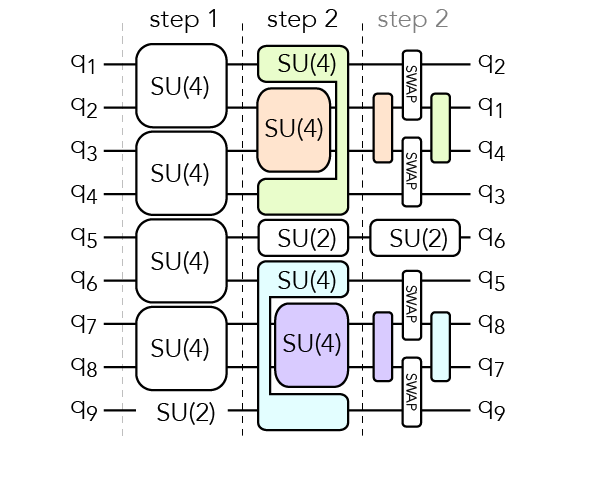
\includegraphics[width=0.7\textwidth]{model_algorithm.png}
\caption{\label{fig:org7e27eec}
Model algorithm example from \cite{Moll_2018}. Each step represents a possible combination of gates considered as \emph{model algorithm}. Notice that step 2 requires a mapping process that is shown afterwards.}
\end{figure}


\begin{description}
\item[{Active qubits (\(\textbf{n}\))}] Number of active qubits in a device of \(N\) qubits for a given algorithm.
\end{description}


\begin{description}
\item[{Effective error rate (\(\epsilon_{eff} \sim 1/(d n)\)).}] It defines how well a device can implement arbitrary pairwise interactions between qubits. \(\epsilon_{eff}\) is the error rate per \emph{model algorithm}, an averaged error over many realizations of depth-one circuits conformed with random combinations of single- and two-qubit gates. It encapsulates errors of both single- and two-qubit gates. And it depends not only on the gate error rates and connectivity, but also on the sophistication of the scheduling algorithm responsible for mapping the model algorithm to the hardware.

\item[{Achievable circuit depth (\(d(N) \simeq \frac{1}{N \epsilon_{eff}}\))}] Maximum circuit depth for which the results, after running it on some device, are correctable and useful.
\end{description}

\begin{description}
\item[{(General) Quantum Volume (\(\tilde{V}_Q = min (N, d(N))^2\))}] quantifies the space-time volume occupied by a model circuit with random two-qubit gates that can be reliably executed on a given device.
\end{description}

\subsection{Runnability}
\label{sec:orgfdc34dc}

After understading the concept of Quantum Volume, we derived some insights and we had ideas motivated by the possibilities that the new metric offers. 
We define the \textbf{runnability} of a given quantum circuit on a device based on the separation of the concepts of \emph{device} Quantum Volume (\(V_Q\)) and \emph{algorithm} Quantum Volume (\(V^a_Q\)).


\subsubsection{Quantum Volume of a device}
\label{sec:org848c2ba}

Following \cite{Bishop_2017,Moll_2018}, we can expand the Quantum Volume general equation (\(\tilde{V}_Q\)) with the other definitions in the previous section and maximize for the biggest possible \(n\) in the device. 
Then, the maximum Quantum Volume that a device could run is defined by:

$$V_Q = \max_{n \le N} \min \left[ n,\frac{1}{n \epsilon_{eff} (n)}\right]^2$$

We define this Quantum Volume as the \emph{device} Quantum Volume. 
In Fig. \ref{fig:deviceQV2} and Fig. \ref{fig:deviceQV1} a graph describing the Quantum Volume as a function of \(n\) and \(\epsilon_{eff}\) is shown.
For this example we are not considering \(\epsilon_{eff} (n)\).
Otherwise it would be a device specific graph and the purpose of this figure is tho show the general behaviour of \(V_Q\).
Note that the axis are in a logarithmic scale in order to show that \(V_Q\) grows exponentially as \(n\) increase and that \(\epsilon_{eff}\) is abruptly detonating \(V_Q\) growth from values smaller than \(10^{-3}\).
Therefore, we outline that the main limit for the \(V_Q\) is the \(\epsilon_{eff}\).

%\begin{figure}

%\centering
\begin{minipage}{.45\textwidth}

\centering

\begin{center}
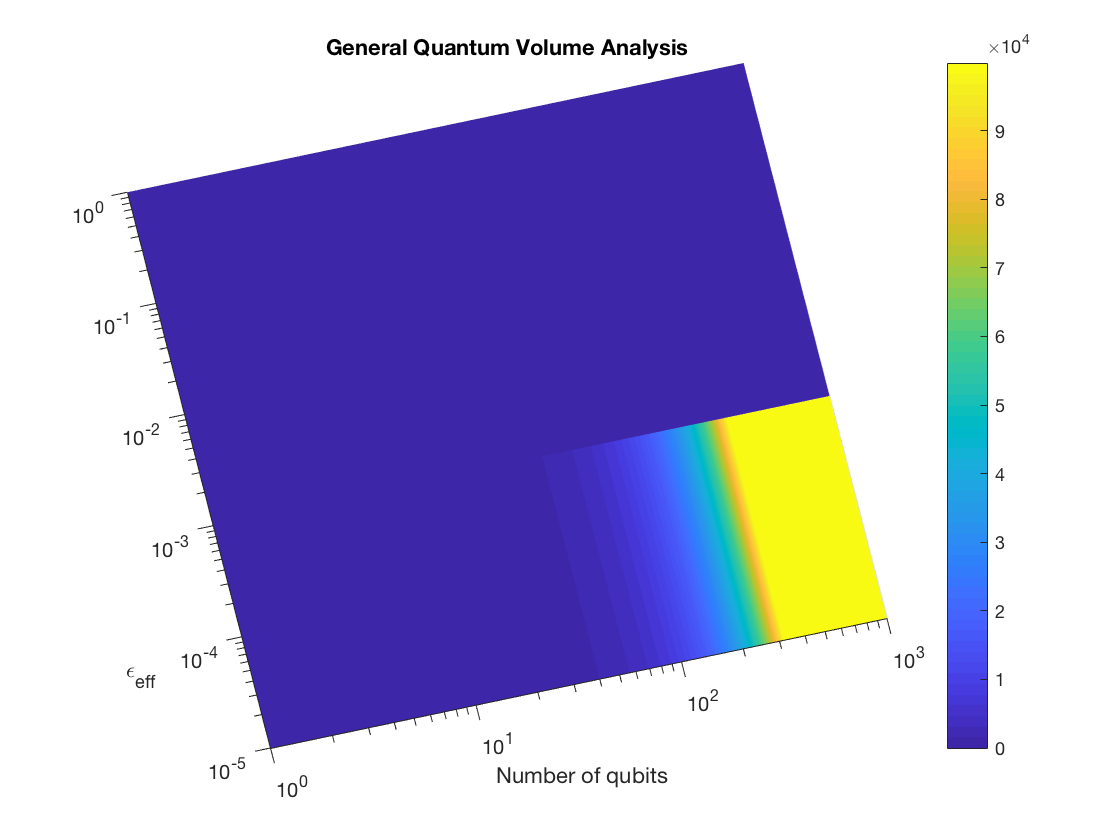
\includegraphics[width=.9\linewidth]{general_QV2.png}
\end{center}

\captionof{figure}{}
\label{fig:deviceQV2}

\end{minipage}%
\hspace{1cm}
\begin{minipage}{.45\textwidth}

\begin{center}
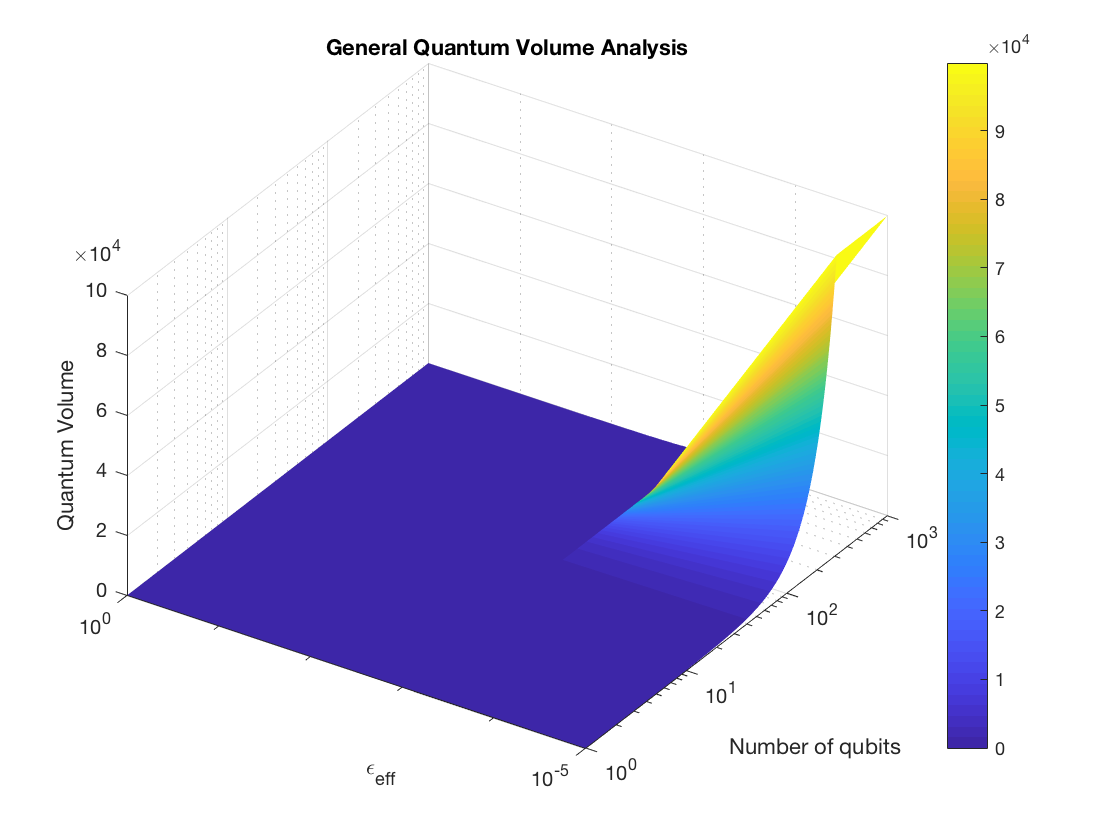
\includegraphics[width=.9\linewidth]{general_QV1.png}
\end{center}

\captionof{figure}{}
\label{fig:deviceQV1}

\end{minipage}%

\subsubsection{Quantum Volume of an algorithm}
\label{sec:orgbcd85a7}

As with \(V_Q\), we initially defined the algorithm's Quantum Volume from the general equation \(\tilde{V}_Q\), although we will later adapt it.

$$V_Q^a = \min \left[ n,d \right]^2$$

Note that \(d\) is not \(d(N)\) but the real depth of the given algorithm.
At the same time, \(n\) is the number of qubits required by the algorithm itself.
One can see how \(d\) and \(n\) are equally important in Fig. \ref{fig:algorithmQV2sym} and Fig. \ref{fig:algorithmQV1sym}.
The growth of both variables causes an equally exponential growth of \(V^a_Q\).

%\begin{figure}

%\centering
\begin{minipage}{.45\textwidth}

\centering

\begin{center}
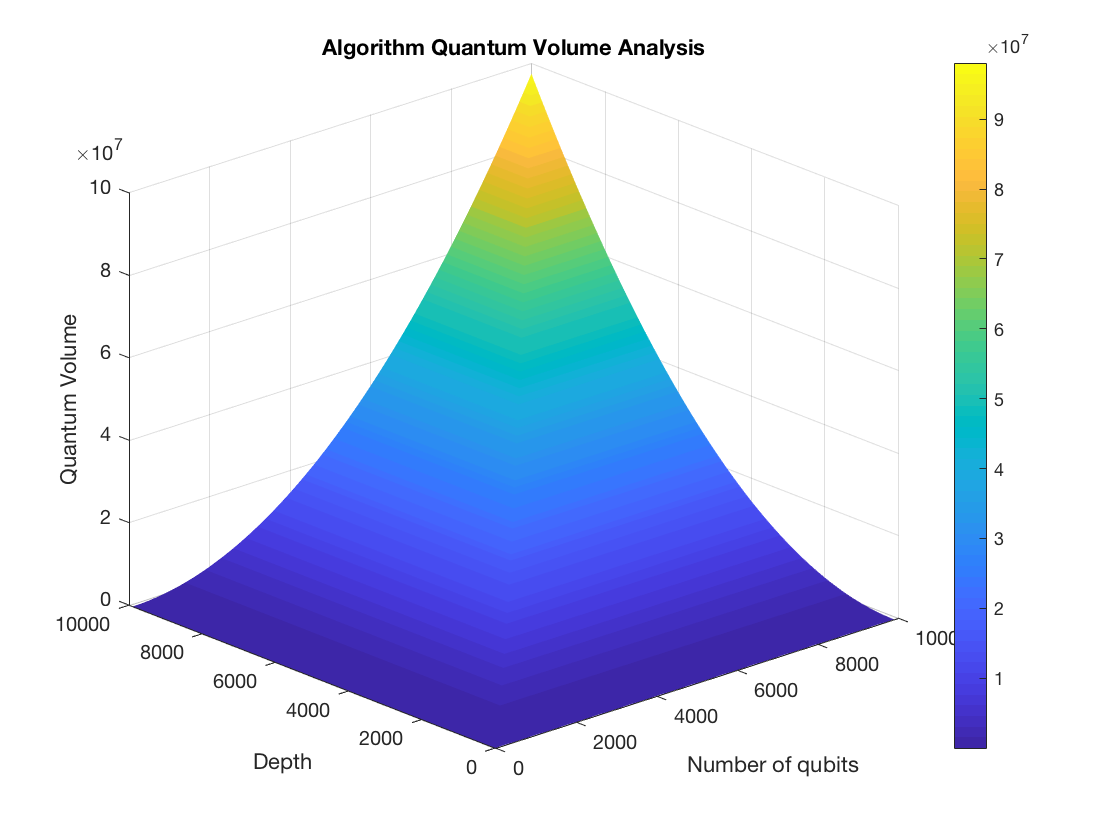
\includegraphics[width=.9\linewidth]{V_q_analysis_sym2.png}
\end{center}

\captionof{figure}{}
\label{fig:algorithmQV2sym}

\end{minipage}%
\hspace{1cm}
\begin{minipage}{.45\textwidth}

\begin{center}
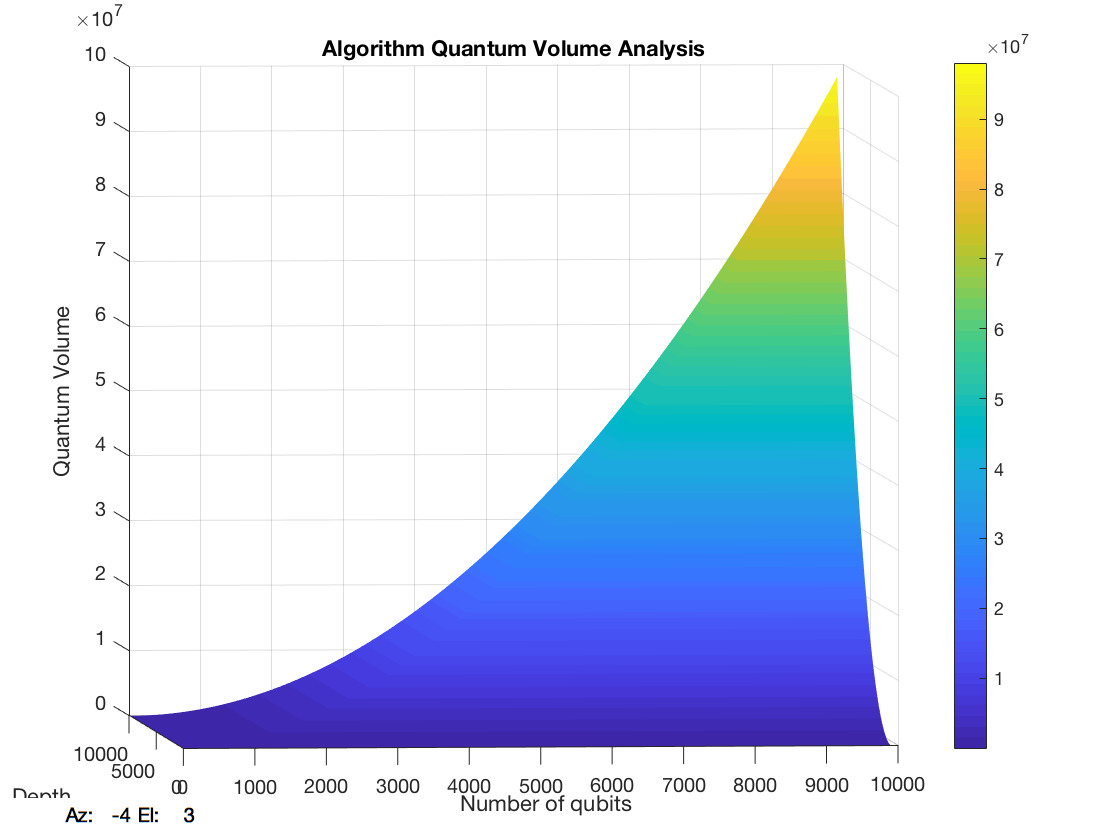
\includegraphics[width=.9\linewidth]{V_q_analysis_sym1.png}
\end{center}

\captionof{figure}{}
\label{fig:algorithmQV1sym}

\end{minipage}%

Fig. \ref{fig:algorithmQV2asym} and Fig. \ref{fig:algorithmQV1asym} present the behaviour of \(V_Q^a\)
focusing in the current most common values for \(n\) and \(d\).
The function shows an asymteric beheviour due to \(d\) is much bigger than \(n\) most of the times.


%\begin{figure}

%\centering
\begin{minipage}{.45\textwidth}

\centering

\begin{center}
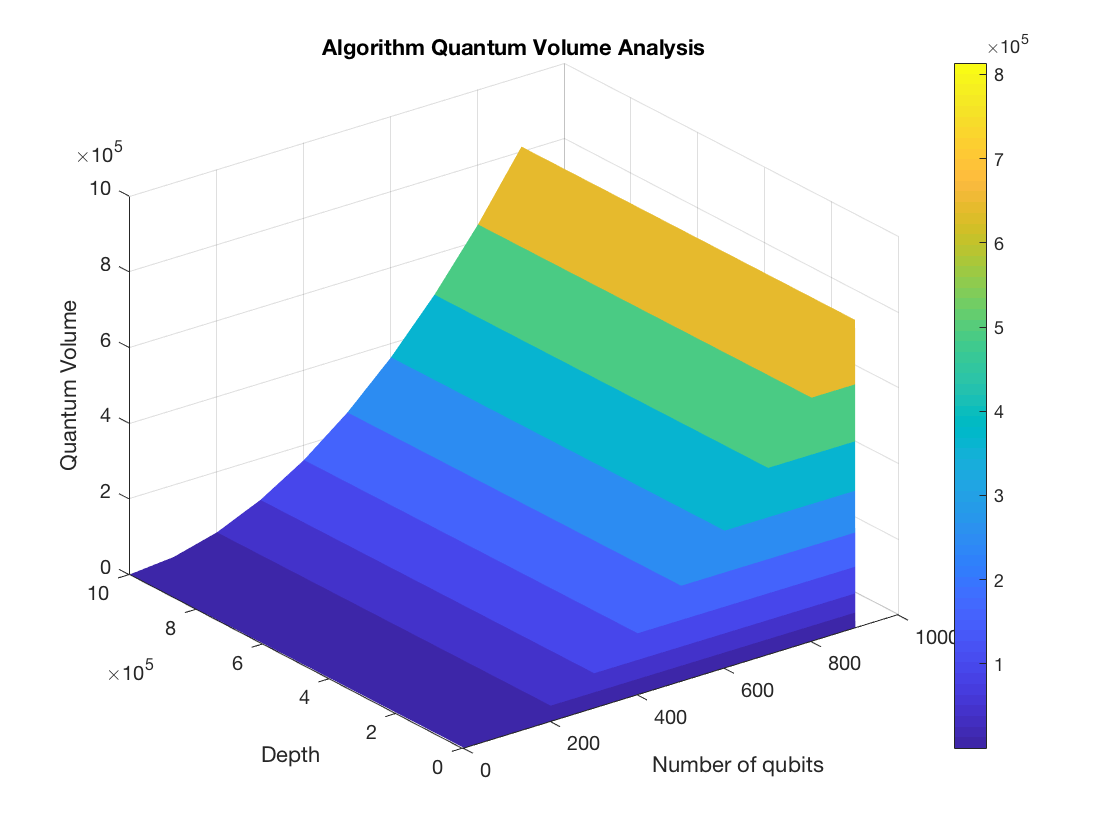
\includegraphics[width=.9\linewidth]{V_q_analysis_asym2.png}
\end{center}

\captionof{figure}{}
\label{fig:algorithmQV2asym}

\end{minipage}%
\hspace{1cm}
\begin{minipage}{.45\textwidth}

\begin{center}
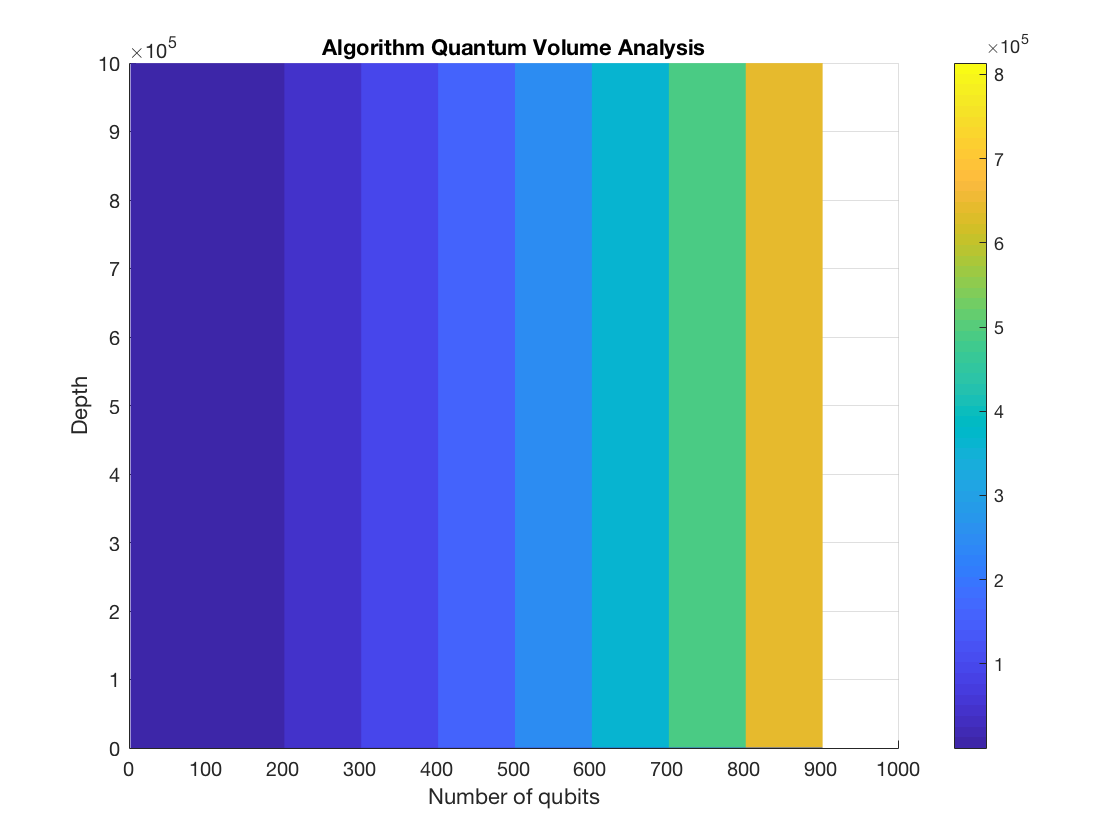
\includegraphics[width=.9\linewidth]{V_q_analysis_asym1.png}
\end{center}

\captionof{figure}{}
\label{fig:algorithmQV1asym}

\end{minipage}%


We aware that this approach has a limitation regarding the mapping of the quantum circuit.
As explained before, \(V_Q\) is able to take into account the sophistication of the mapping procedure.
It is inherited in the \emph{model algorithm}.
But, in this case, the \(V^a_Q\) of an algorithm before and after mapping will remain the same.
After mapping an algorithm, the usual effect is an increase in the depth or the number of operations.
Rare mapping methods consider the qubit addition in the technique.
And, even considering it, \(n\) is not often growing too much in comparison with \(d\).
In the current NISQ era, the quantum circuits need much less qubits than depth.
Therefore, most of the times, the minimum value between \(n\) and \(d\) will be \(n\).
As soon as \(V^a_Q\) is taking into account the minimum of them and the mapping procedure affects mostly to \(d\) we can conclude that this definition of \(V^a_Q\) is not considering the mapping in its results.

A simplified solution for this problem would be the \(V^a_Q\) definition as the multiplication of \(n\) and \(d\).
Unfortunately, this approach has several drawbacks as well.
As Moll et al. point out \cite{Moll_2018}, extreme cases of high \(n\) and low \(d\) -- or the other way around -- lead to inconsistencies of the multiplication metric.
Considering that most of our work is not going to be in any of these extreme cases and that we can avoid those outliers, we consider the definition of the algorithm's Quantum Volume as:

$$V_Q^a =  n \times d$$

%\begin{figure}

%\centering
\begin{minipage}{.45\textwidth}

\centering

\begin{center}
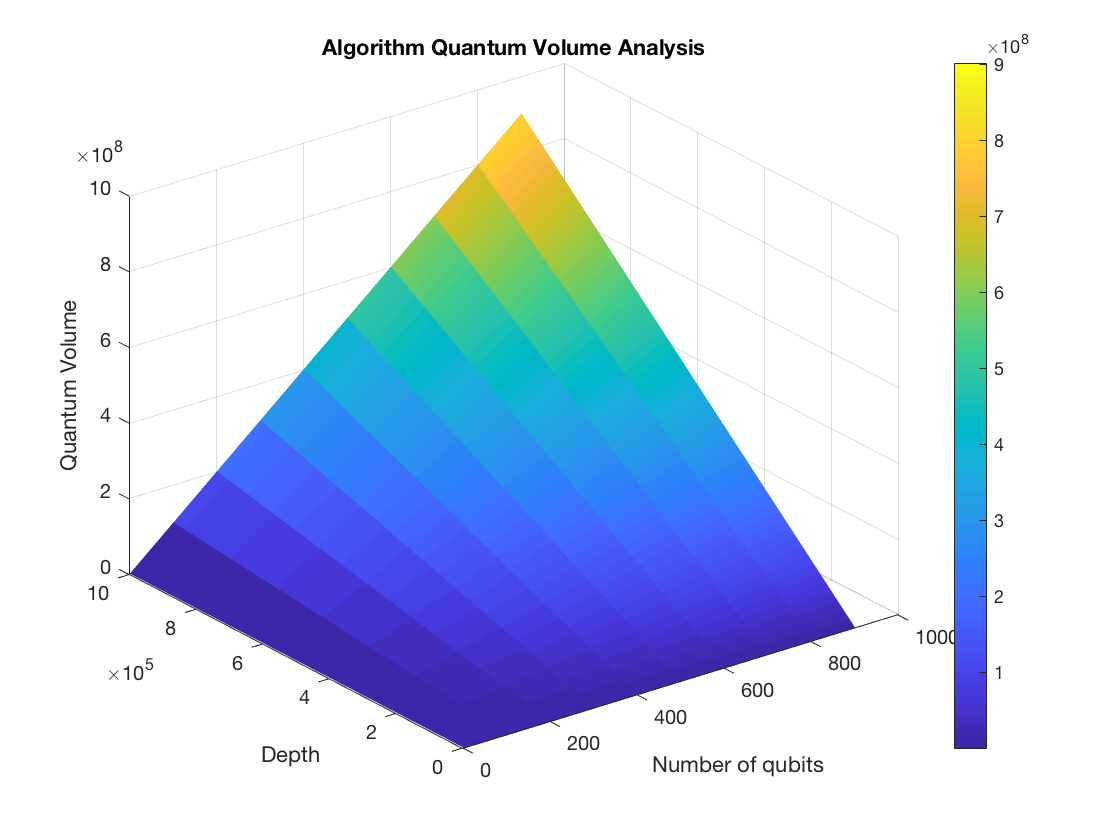
\includegraphics[width=.9\linewidth]{V_q_analysis_mult2.png}
\end{center}

\captionof{figure}{}
\label{fig:algorithmmultQV2}

\end{minipage}%
\hspace{1cm}
\begin{minipage}{.45\textwidth}

\begin{center}
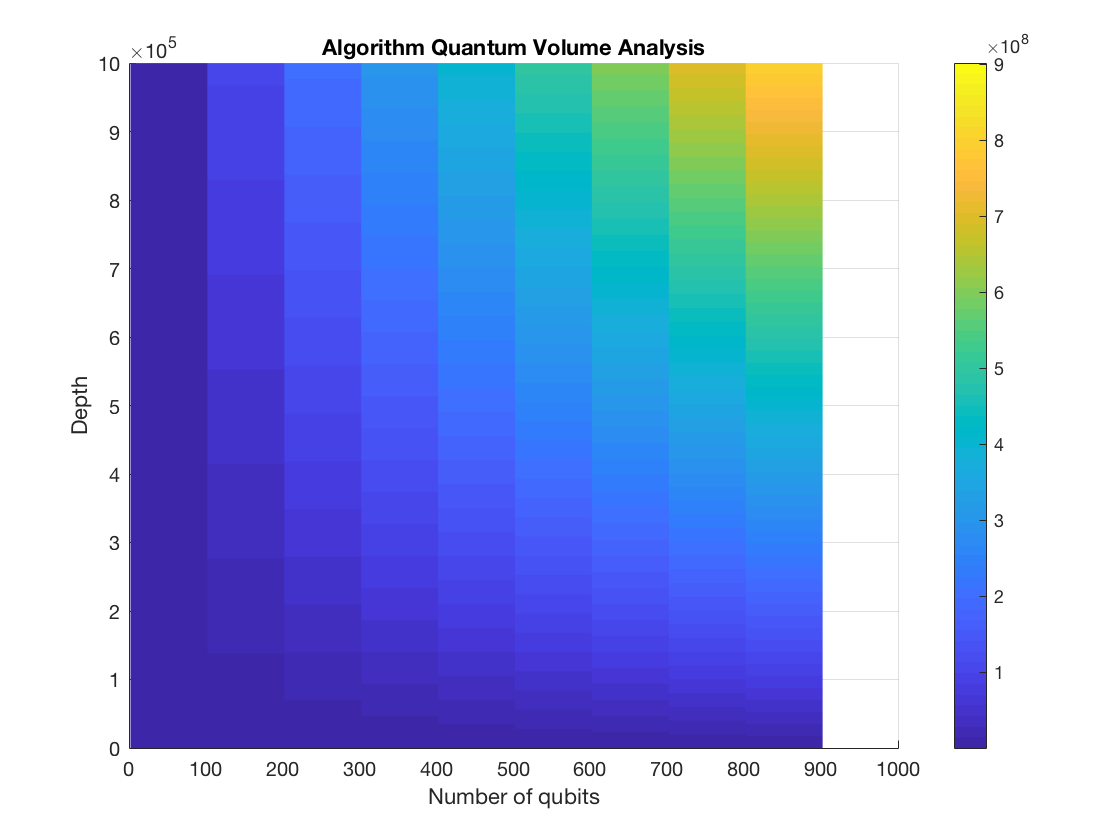
\includegraphics[width=.9\linewidth]{V_q_analysis_mult1.png}
\end{center}

\captionof{figure}{}
\label{fig:algorithmmultQV1}

\end{minipage}%

\subsubsection{Runnability}
\label{sec:org5acc633}

Finally, once the Quantum Volume of device and algorithm are stated, we define runnability as the condition for which the \(V_Q\) should be bigger than \(V^a_Q\).
That is the condition that the computational power of the device should be bigger than the computational power required by the algorithm.

$$\text{Runnable if: } V_Q > V^a_Q$$

For instance, in order to understand this concept, one may imagine the process of checking, whether or not, some cube with a given volume -- representing the algorithm -- would fit in a box -- the device --.
If the "algorithm's box" volume is smaller than the volume of the device's box, the algorithm's box will fit inside.

Indeed, one acceptable criticism of this definition is that, as \(V_Q\) and \(V^a_Q\) are finally defined in the previous sections, it seems that it is not really fair to compare them.
But, as soon as the general behaviour of the final and the initial \(V^a_Q\) is the same -- one can see in the Fig. \ref{fig:algorithmQV1sym} and Fig. \ref{fig:algorithmmultQV1} -- and that the final definition tends to be bigger than the initial one -- so it is defining a more restrictive and exigent scenario -- we believe that this definition of runnability mathematically correct and useful.

Therefore, we define runnability as the condition of:

$$\max_{n \le N} \min \left[ n,\frac{1}{n \epsilon_{eff} (n)}\right]^2 > n \times d$$

\section{Methodology}
\label{sec:orgba571b7}

\bibliography{../thesis_plan}
\bibliographystyle{plain}
\end{document}
